\chapter[APÊNDICE \ref{Ap:DinBeam}]{Viga engastada em problema dinâmico}
\label{Ap:DinBeam}

Para verificação do código implementado em problemas dinâmicos, estudou-se  primeiramente o comportamento de uma viga engastada em uma de suas extremidades e sujeita a uma carga $P$ aplicada na extremidade oposta, conforme ilustrado na Figura \ref{fig:viga1}. As dimensões da viga são: comprimento $L=60$ dm, altura $h=3$ dm e largura $b=1$ dm. A força aplicada possui intensidade $P=1,25\times10^{-4}$ Mg$\cdot$dm/(ms)² $H(t)$, sendo $H(t)$ a função de Heavside. O material que compõe a viga possui módulo de Young $E=20$ Mg/[dm$\cdot$(ms)²], coeficiente de Poisson nulo e massa específica $\rho=7\times10^{-3}$ Mg/dm³. O intervalo de tempo analisado foi $t\in[0;675]$ ms discretizado em passos de tempo $\Delta t=0,3377$. A malha de elementos finitos utilizada conta com 32 elementos triangulares de aproximação quadrática, com um total de 693 graus de liberdade, a qual pode ser observada na Figura \ref{fig:viga1-mesh}.

\begin{figure}[h!]
    \centering
    \caption{Desenho esquemático da viga simulada.}
    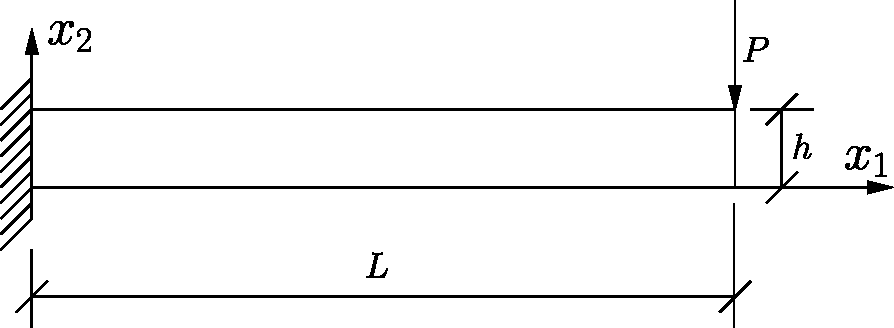
\includegraphics[width=0.5\linewidth]{Figuras/vigas/viga1.pdf}
    \\Fonte: Autoria Própria (\the\year).
    \label{fig:viga1}
\end{figure}

\begin{figure}[h!]
    \centering
    \caption{Malha utilizada na simulação da viga.}
    
\includegraphics[width=\linewidth]{Figuras/vigas/mesh1.png}
    \\Fonte: Autoria Própria (\the\year).
    \label{fig:viga1-mesh}
\end{figure}

A modelagem realizada considerou a altura $H$ como a espessura do elemento de casca, sendo a força atuante nessa mesma direção. Assim, observou-se o deslocamento vertical no ponto de aplicação da força. Os resultados obtidos foram comparados com aqueles alcançados a partir de uma modelagem no \textit{software} ANSYS utilizando elementos sólidos 183. a Figura \ref{fig:res-viga1} apresenta os resultados calculados.

\begin{figure}[h!]
    \centering
    \caption{Deslocamento vertical no ponto de aplicação da força ao longo do tempo.}
    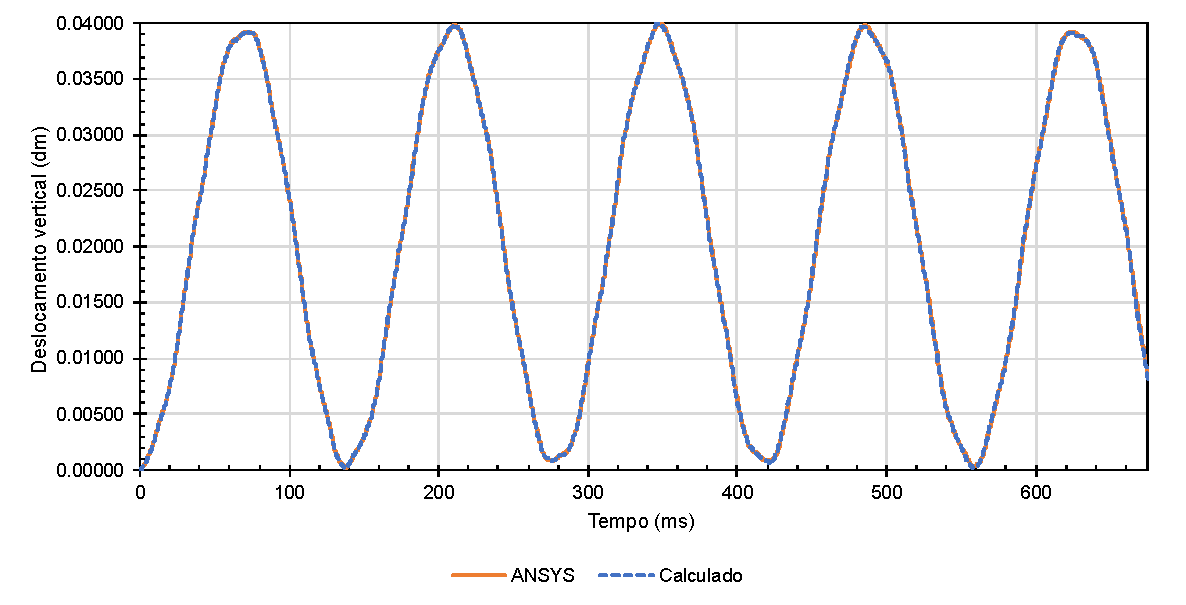
\includegraphics[width=\linewidth]{Figuras/vigas/res1.pdf}
    \\Fonte: Autoria Própria (\the\year).
    \label{fig:res-viga1}
\end{figure}

Observa-se nesse caso uma boa concordância entre os resultados apresentados pelo ANSYS e os obtidos pelo código desenvolvido, sendo verificada a eficácia nesse exemplo.

Outro exemplo trata-se de uma viga biengastada com uma carga aplicada em seu centro, conforme mostrado na Figura \ref{fig:viga2}. Nesse exemplo considerou-se um comprimento $L=20$ in, com seção transversal de $b\times h=1,0\times0,125$ in². O material que constitui a viga possui módulo de Young $E=3\times10^{7}$ lb/in², coeficiente de Poisson nulo e massa específica de $\rho=2,6\times10^{-4}$ lb$\cdot$s²/in$^4$. A força aplicada foi de $P=640$ lb constante durante todo o período de análise, de $t\in[0;5]$ ms, o qual foi discretizado em passos de tempo de $\Delta t=25\ \mu$ s. A malha de elementos finitos (Figura \ref{fig:viga2-mesh}) possui 132 elementos triangulares de aproximação quadrática, totalizando 2331 graus de liberdade. A espessura do elemento de casca foi considerado como a direção da altura $H$ da viga.

\begin{figure}[h!]
    \centering
    \caption{Desenho esquemático da viga biengastada simulada.}
    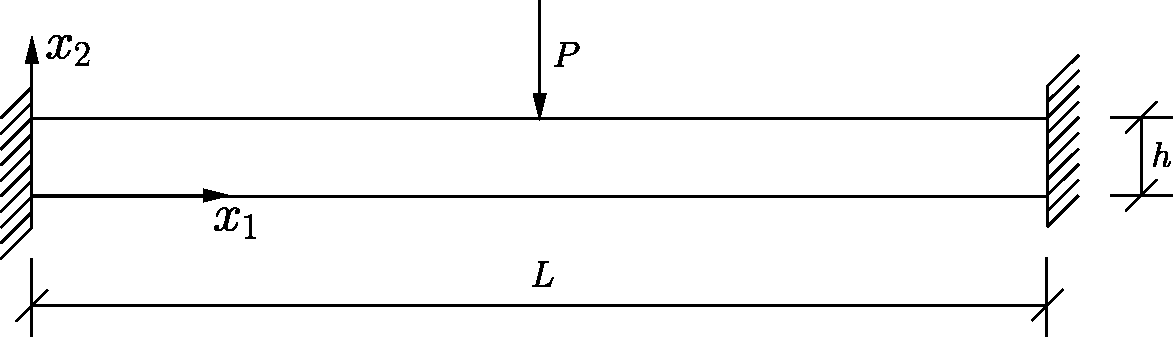
\includegraphics[width=0.6\linewidth]{Figuras/vigas/viga2.pdf}
    \\Fonte: Autoria Própria (\the\year).
    \label{fig:viga2}
\end{figure}

\begin{figure}[h!]
    \centering
    \caption{Malha utilizada na simulação da viga biengastada.}
    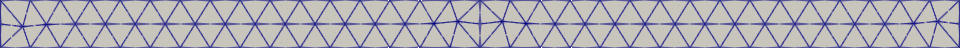
\includegraphics[width=\linewidth]{Figuras/vigas/mesh2.png}
    \\Fonte: Autoria Própria (\the\year).
    \label{fig:viga2-mesh}
\end{figure}

Os resultados calculados foram comparados com os apresentados pelo ANSYS, a partir do elemento 183, e por \cite{mondkar1977ansa}. A Figura \ref{fig:res-viga2} exibe os resultados obtidos.

\begin{figure}[h!]
    \centering
    \caption{Deslocamento vertical no centro da viga biengastada ao longo do tempo.}
    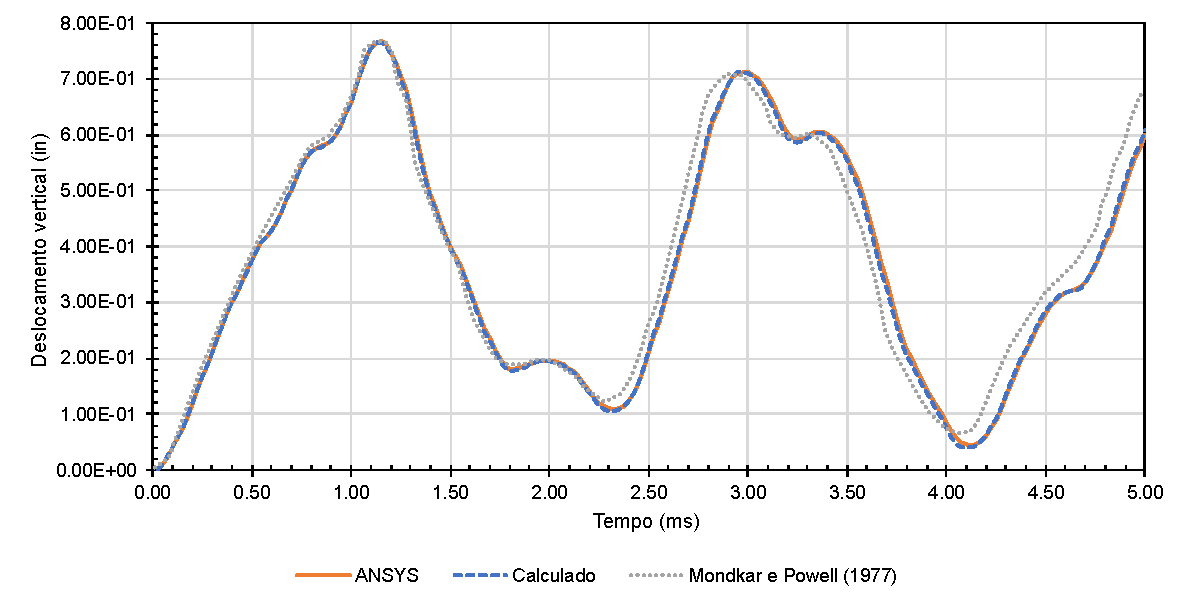
\includegraphics[width=\linewidth]{Figuras/vigas/res2.pdf}
    \\Fonte: Autoria Própria (\the\year).
    \label{fig:res-viga2}
\end{figure}

Verifica-se uma boa concordância entre os resultados obtidos pela análise por ambos os valores de referência, sendo assim, averiguada a eficácia do código nesse exemplo.